% Created by tikzDevice version 0.10.1 on 2017-04-13 19:14:03
% !TEX encoding = UTF-8 Unicode
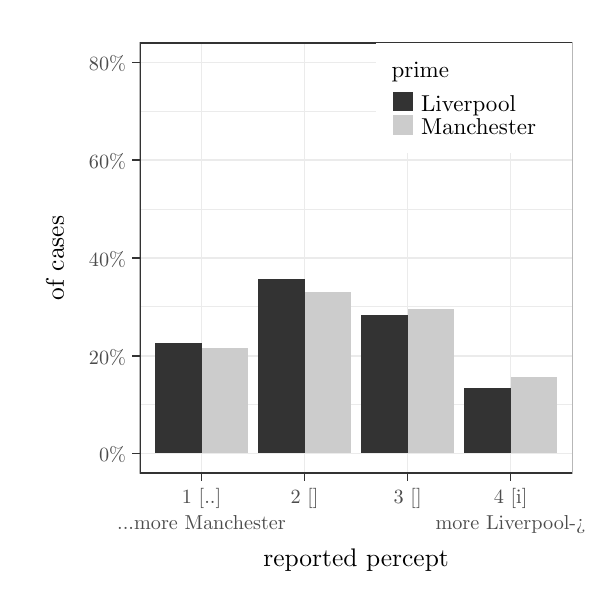
\begin{tikzpicture}[x=1pt,y=1pt]
\definecolor{fillColor}{RGB}{255,255,255}
\path[use as bounding box,fill=fillColor,fill opacity=0.00] (0,0) rectangle (202.36,202.36);
\begin{scope}
\path[clip] (  0.00,  0.00) rectangle (202.36,202.36);
\definecolor{drawColor}{RGB}{255,255,255}
\definecolor{fillColor}{RGB}{255,255,255}

\path[draw=drawColor,line width= 0.6pt,line join=round,line cap=round,fill=fillColor] (  0.00,  0.00) rectangle (202.36,202.36);
\end{scope}
\begin{scope}
\path[clip] ( 40.49, 41.42) rectangle (196.86,196.86);
\definecolor{fillColor}{RGB}{255,255,255}

\path[fill=fillColor] ( 40.49, 41.42) rectangle (196.86,196.86);
\definecolor{drawColor}{gray}{0.92}

\path[draw=drawColor,line width= 0.3pt,line join=round] ( 40.49, 66.15) --
	(196.86, 66.15);

\path[draw=drawColor,line width= 0.3pt,line join=round] ( 40.49,101.48) --
	(196.86,101.48);

\path[draw=drawColor,line width= 0.3pt,line join=round] ( 40.49,136.80) --
	(196.86,136.80);

\path[draw=drawColor,line width= 0.3pt,line join=round] ( 40.49,172.13) --
	(196.86,172.13);

\path[draw=drawColor,line width= 0.6pt,line join=round] ( 40.49, 48.49) --
	(196.86, 48.49);

\path[draw=drawColor,line width= 0.6pt,line join=round] ( 40.49, 83.81) --
	(196.86, 83.81);

\path[draw=drawColor,line width= 0.6pt,line join=round] ( 40.49,119.14) --
	(196.86,119.14);

\path[draw=drawColor,line width= 0.6pt,line join=round] ( 40.49,154.47) --
	(196.86,154.47);

\path[draw=drawColor,line width= 0.6pt,line join=round] ( 40.49,189.79) --
	(196.86,189.79);

\path[draw=drawColor,line width= 0.6pt,line join=round] ( 62.82, 41.42) --
	( 62.82,196.86);

\path[draw=drawColor,line width= 0.6pt,line join=round] (100.06, 41.42) --
	(100.06,196.86);

\path[draw=drawColor,line width= 0.6pt,line join=round] (137.29, 41.42) --
	(137.29,196.86);

\path[draw=drawColor,line width= 0.6pt,line join=round] (174.52, 41.42) --
	(174.52,196.86);
\definecolor{fillColor}{gray}{0.80}

\path[fill=fillColor] ( 62.82, 48.49) rectangle ( 79.58, 86.73);
\definecolor{fillColor}{gray}{0.20}

\path[fill=fillColor] ( 46.07, 48.49) rectangle ( 62.82, 88.31);
\definecolor{fillColor}{gray}{0.80}

\path[fill=fillColor] (100.06, 48.49) rectangle (116.81,106.90);
\definecolor{fillColor}{gray}{0.20}

\path[fill=fillColor] ( 83.30, 48.49) rectangle (100.06,111.43);
\definecolor{fillColor}{gray}{0.80}

\path[fill=fillColor] (137.29, 48.49) rectangle (154.04,100.64);
\definecolor{fillColor}{gray}{0.20}

\path[fill=fillColor] (120.53, 48.49) rectangle (137.29, 98.59);
\definecolor{fillColor}{gray}{0.80}

\path[fill=fillColor] (174.52, 48.49) rectangle (191.27, 76.30);
\definecolor{fillColor}{gray}{0.20}

\path[fill=fillColor] (157.76, 48.49) rectangle (174.52, 72.25);
\definecolor{drawColor}{gray}{0.20}

\path[draw=drawColor,line width= 0.6pt,line join=round,line cap=round] ( 40.49, 41.42) rectangle (196.86,196.86);
\end{scope}
\begin{scope}
\path[clip] (  0.00,  0.00) rectangle (202.36,202.36);
\definecolor{drawColor}{gray}{0.30}

\node[text=drawColor,anchor=base east,inner sep=0pt, outer sep=0pt, scale=  0.73] at ( 35.54, 45.46) {0{\%}};

\node[text=drawColor,anchor=base east,inner sep=0pt, outer sep=0pt, scale=  0.73] at ( 35.54, 80.78) {20{\%}};

\node[text=drawColor,anchor=base east,inner sep=0pt, outer sep=0pt, scale=  0.73] at ( 35.54,116.11) {40{\%}};

\node[text=drawColor,anchor=base east,inner sep=0pt, outer sep=0pt, scale=  0.73] at ( 35.54,151.44) {60{\%}};

\node[text=drawColor,anchor=base east,inner sep=0pt, outer sep=0pt, scale=  0.73] at ( 35.54,186.76) {80{\%}};
\end{scope}
\begin{scope}
\path[clip] (  0.00,  0.00) rectangle (202.36,202.36);
\definecolor{drawColor}{gray}{0.20}

\path[draw=drawColor,line width= 0.6pt,line join=round] ( 37.74, 48.49) --
	( 40.49, 48.49);

\path[draw=drawColor,line width= 0.6pt,line join=round] ( 37.74, 83.81) --
	( 40.49, 83.81);

\path[draw=drawColor,line width= 0.6pt,line join=round] ( 37.74,119.14) --
	( 40.49,119.14);

\path[draw=drawColor,line width= 0.6pt,line join=round] ( 37.74,154.47) --
	( 40.49,154.47);

\path[draw=drawColor,line width= 0.6pt,line join=round] ( 37.74,189.79) --
	( 40.49,189.79);
\end{scope}
\begin{scope}
\path[clip] (  0.00,  0.00) rectangle (202.36,202.36);
\definecolor{drawColor}{gray}{0.20}

\path[draw=drawColor,line width= 0.6pt,line join=round] ( 62.82, 38.67) --
	( 62.82, 41.42);

\path[draw=drawColor,line width= 0.6pt,line join=round] (100.06, 38.67) --
	(100.06, 41.42);

\path[draw=drawColor,line width= 0.6pt,line join=round] (137.29, 38.67) --
	(137.29, 41.42);

\path[draw=drawColor,line width= 0.6pt,line join=round] (174.52, 38.67) --
	(174.52, 41.42);
\end{scope}
\begin{scope}
\path[clip] (  0.00,  0.00) rectangle (202.36,202.36);
\definecolor{drawColor}{gray}{0.30}

\node[text=drawColor,anchor=base,inner sep=0pt, outer sep=0pt, scale=  0.73] at ( 62.82, 30.41) {1 [..]};

\node[text=drawColor,anchor=base,inner sep=0pt, outer sep=0pt, scale=  0.73] at ( 62.82, 20.91) { ...more Manchester};

\node[text=drawColor,anchor=base,inner sep=0pt, outer sep=0pt, scale=  0.73] at (100.06, 30.41) {2 []};

\node[text=drawColor,anchor=base,inner sep=0pt, outer sep=0pt, scale=  0.73] at (137.29, 30.41) {3 []};

\node[text=drawColor,anchor=base,inner sep=0pt, outer sep=0pt, scale=  0.73] at (174.52, 30.41) {4 [i]};

\node[text=drawColor,anchor=base,inner sep=0pt, outer sep=0pt, scale=  0.73] at (174.52, 20.91) { more Liverpool->};
\end{scope}
\begin{scope}
\path[clip] (  0.00,  0.00) rectangle (202.36,202.36);
\definecolor{drawColor}{RGB}{0,0,0}

\node[text=drawColor,anchor=base,inner sep=0pt, outer sep=0pt, scale=  0.92] at (118.67,  7.83) {reported percept};
\end{scope}
\begin{scope}
\path[clip] (  0.00,  0.00) rectangle (202.36,202.36);
\definecolor{drawColor}{RGB}{0,0,0}

\node[text=drawColor,rotate= 90.00,anchor=base,inner sep=0pt, outer sep=0pt, scale=  0.92] at ( 13.08,119.14) {of cases};
\end{scope}
\begin{scope}
\path[clip] (  0.00,  0.00) rectangle (202.36,202.36);
\definecolor{fillColor}{RGB}{255,255,255}

\path[fill=fillColor] (125.78,157.18) rectangle (196.86,196.86);
\end{scope}
\begin{scope}
\path[clip] (  0.00,  0.00) rectangle (202.36,202.36);
\definecolor{drawColor}{RGB}{0,0,0}

\node[text=drawColor,anchor=base west,inner sep=0pt, outer sep=0pt, scale=  0.83] at (131.47,184.28) {prime};
\end{scope}
\begin{scope}
\path[clip] (  0.00,  0.00) rectangle (202.36,202.36);
\definecolor{fillColor}{RGB}{255,255,255}

\path[fill=fillColor] (131.47,171.41) rectangle (140.00,179.94);
\end{scope}
\begin{scope}
\path[clip] (  0.00,  0.00) rectangle (202.36,202.36);
\definecolor{fillColor}{gray}{0.20}

\path[fill=fillColor] (132.18,172.12) rectangle (139.29,179.23);
\end{scope}
\begin{scope}
\path[clip] (  0.00,  0.00) rectangle (202.36,202.36);
\definecolor{fillColor}{RGB}{255,255,255}

\path[fill=fillColor] (131.47,162.87) rectangle (140.00,171.41);
\end{scope}
\begin{scope}
\path[clip] (  0.00,  0.00) rectangle (202.36,202.36);
\definecolor{fillColor}{gray}{0.80}

\path[fill=fillColor] (132.18,163.58) rectangle (139.29,170.70);
\end{scope}
\begin{scope}
\path[clip] (  0.00,  0.00) rectangle (202.36,202.36);
\definecolor{drawColor}{RGB}{0,0,0}

\node[text=drawColor,anchor=base west,inner sep=0pt, outer sep=0pt, scale=  0.83] at (142.17,172.23) {Liverpool};
\end{scope}
\begin{scope}
\path[clip] (  0.00,  0.00) rectangle (202.36,202.36);
\definecolor{drawColor}{RGB}{0,0,0}

\node[text=drawColor,anchor=base west,inner sep=0pt, outer sep=0pt, scale=  0.83] at (142.17,163.70) {Manchester};
\end{scope}
\end{tikzpicture}
